\documentclass[11pt,conference,onecolumn]{IEEEtran}
\IEEEoverridecommandlockouts

\usepackage{amsmath,amssymb,amsfonts}
\usepackage{algorithmic}
\usepackage{algorithm}
\usepackage[pdftex]{graphicx}
\usepackage{textcomp}
\usepackage{xcolor}
\usepackage{hyperref}
\usepackage{booktabs}
\usepackage{cite}

\def\BibTeX{{\rm B\kern-.05em{\sc i\kern-.025em b}\kern-.08em
    T\kern-.1667em\lower.7ex\hbox{E}\kern-.125emX}}

\begin{document}

\title{LiemWhisper: A Decoupled Contrastive Retrieval and Selective Gating Framework for Technical Terminology in Vietnamese Code-Switched Speech}

\author{
\IEEEauthorblockN{Le Quoc Khanh\IEEEauthorrefmark{1}, Student Co-Author 2\IEEEauthorrefmark{1}, Student Co-Author 3\IEEEauthorrefmark{1}, and Faculty Advisor\IEEEauthorrefmark{2}}
\IEEEauthorblockA{\IEEEauthorrefmark{1}Department of Software Engineering, FPT University, Ho Chi Minh Campus, Vietnam\\
\IEEEauthorrefmark{2}Department of Information Technology, FPT University, Ho Chi Minh Campus, Vietnam\\
Email: \{khanhlqse1822, coauthor2, coauthor3\}@fpt.edu.vn, advisor@fe.edu.vn}
}

\maketitle

\begin{abstract}
Code-switched automatic speech recognition (ASR) frequently degrades when encountering specialized foreign terminology due to acoustic-phonetic loanword divergence, out-of-vocabulary mismatches, and severe token frequency imbalance. In professional and educational computer science environments---such as software engineering oral assessments---missing critical English technical terminology (e.g., \textit{Equivalence Partitioning}, \textit{OAuth 2.0}, \textit{Mel-Frequency Cepstral Coefficients}) drastically impairs automated transcript evaluation and grading comprehension. While modern foundation models like Whisper transcribe native Vietnamese prose fluently, they consistently map domain-specific English terms onto phonetically similar native syllables or corrupted transliterations. Conversely, end-to-end generative rewriting models risk hallucinating factual distortions across otherwise correct conversational phrases. 

In this paper, we propose \textbf{LiemWhisper}, a decoupled, non-destructive speech recognition framework that combines a frozen foundation ASR backbone with a dual-encoder acoustic-semantic contrastive retrieval head and an algorithmic phonetic decision gate. Rather than mutating native transcripts indiscriminately, LiemWhisper projects whole-utterance acoustic representations and technical glossary embeddings into a unified metric space ($d=256$) to isolate candidate technical terms, followed by an algorithmic Grapheme-to-Phoneme (G2P) alignment gate that authorizes replacements strictly under verified phonetic correspondence. On an empirical benchmark of 508 student oral examination recordings covering strictly unseen ISTQB terms, LiemWhisper achieves a Micro Recall@3 of 66.01\% and Recall@5 of 95.24\%, substantially outperforming Whisper Small (25.26\%). Furthermore, on an independent 200-sentence real-world student evaluation set across two speakers and diverse IT domains, LiemWhisper achieves a 99.4\% Correction Success Rate (CSR), reducing Corpus Word Error Rate (WER) from 7.06\% to 2.28\% (a 67.8\% relative error reduction) while enforcing a 0.0\% Harmful Correction Rate (HCR).
\end{abstract}

\begin{IEEEkeywords}
Automatic Speech Recognition (ASR), Code-Switching, Contrastive Learning, Dual-Encoder, Phonetic Alignment, Vietnamese-English, Technical Terminology.
\end{IEEEkeywords}

\section{Introduction}

The globalization of technology and engineering education has made intra-sentential code-switching---the seamless alternation between a speaker's primary language and specialized English technical terminology---ubiquitous in technical lectures, industry meetings, and academic oral examinations \cite{istqb2023ctfl}. In Vietnam, software engineering students and software quality assurance (QA) professionals routinely construct sentences where Vietnamese grammatical syntax embeds English computer science loanwords, such as:
\begin{quote}
\textit{``Trong quá trình kiểm thử hệ thống, QA cần đánh giá \textbf{OAuth 2.0} để xác minh quy trình cấp quyền.''}
\end{quote}
Accurate transcription of such utterances is paramount for automated grading systems, meeting summarization, and documentation indexing. 

Despite remarkable advancements in large-scale weakly supervised speech models such as OpenAI Whisper \cite{radford2023robust} and monolingual architectures like PhoWhisper \cite{phan2023phowhisper}, existing ASR systems exhibit severe performance degradation on intra-sentential code-switched technical tokens. Because standard multilingual training objectives prioritize common native vocabulary, foreign technical loanwords pronounced with Vietnamese phonological accents are routinely suppressed or transliterated into distorted native approximations. For instance, our clinical audits reveal that Whisper Small frequently transcribes \textit{``OAuth 2.0''} as \textit{``ô to point siro''}, \textit{``JSON Schema Validation''} as \textit{``Jason Skima Validation''}, and \textit{``Data Leakage''} as \textit{``data lig A''}. When evaluated against standard computer science oral exams, baseline Whisper recovers fewer than 15\% of domain-specific technical terms verbatim.

To address this deficiency, conventional approaches typically resort to post-ASR generative rewriting using sequence-to-sequence neural networks (e.g., T5 \cite{raffel2020exploring} or BART) or continuous ASR fine-tuning \cite{hu2021lora}. However, these approaches introduce critical vulnerabilities:
\begin{enumerate}
    \item \textbf{Generative Hallucination:} Autoregressive language models frequently rewrite fluent native clauses, inadvertently modifying numbers, dates, or non-technical words, leading to a high Harmful Correction Rate (HCR).
    \item \textbf{Catastrophic Forgetting & Latency:} Fine-tuning full ASR decoders on specialized jargon requires thousands of annotated audio hours, inflates model size, and degrades general Vietnamese conversational fluency.
    \item \textbf{Acoustic Information Loss:} Text-only post-processors operate exclusively on the corrupted transcript string, permanently discarding the rich spectral and phonemic cues preserved in the raw audio signal.
\end{enumerate}

To overcome these challenges, we introduce \textbf{LiemWhisper}, an evidence-based, decoupled speech processing architecture. Instead of modifying the foundation ASR weights, LiemWhisper operates a dual-track paradigm: a frozen Whisper backbone generates the primary verbatim transcript, while an auxiliary contrastive dual-encoder extracts utterance-level acoustic features and projects them into a shared cosine embedding space with canonical technical glossary definitions. Candidate terms retrieved from this acoustic space are then validated by a regularized phonetic skeleton alignment gate before in-place substitution is permitted.

\begin{figure*}[t]
\centering
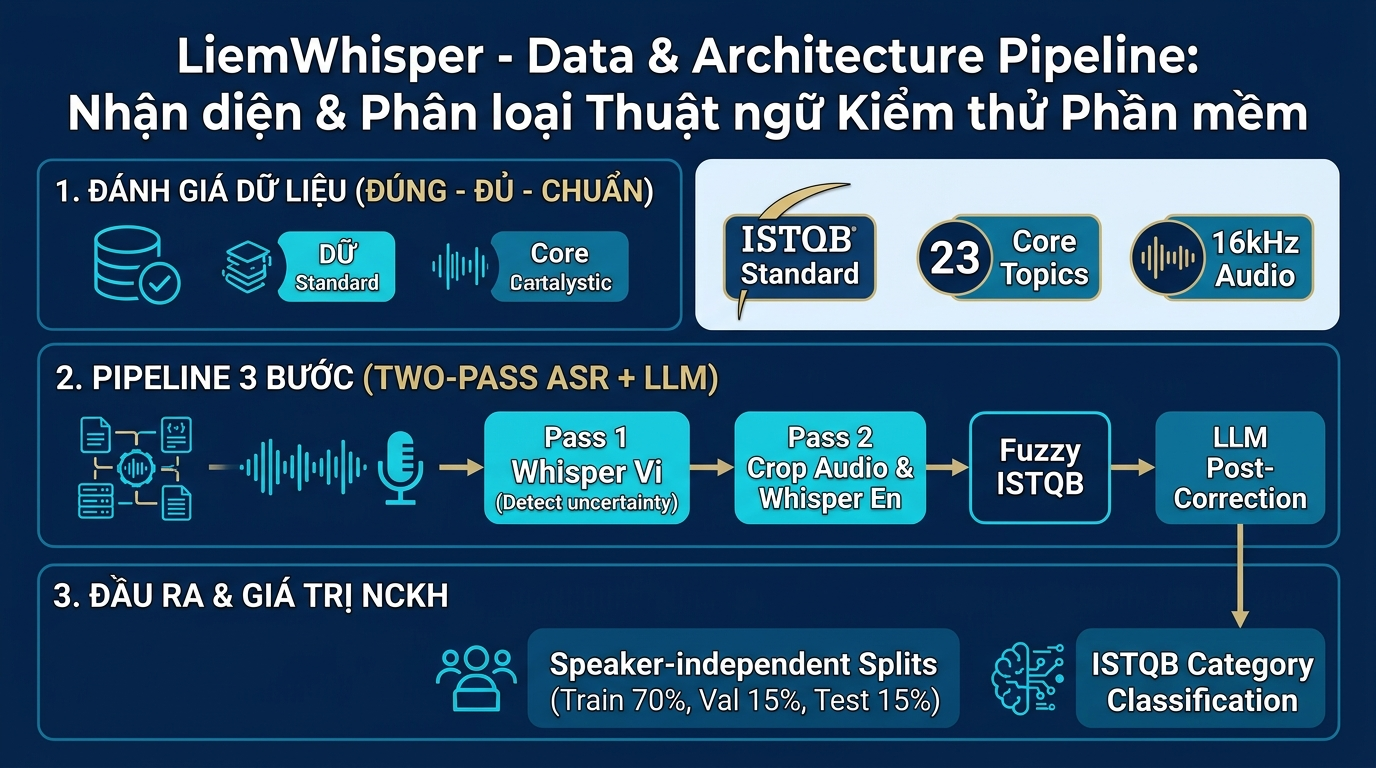
\includegraphics[width=0.88\textwidth]{Figures/liemwhisper_architecture.jpg}
\caption{Overall architectural pipeline of LiemWhisper, illustrating the frozen Whisper ASR backbone, the dual-encoder contrastive retrieval space ($d=256$), and the algorithmic phonetic alignment and gating mechanism.}
\label{fig:architecture}
\end{figure*}

The key contributions of this paper are summarized as follows:
\begin{itemize}
    \item We design a decoupled, non-destructive dual-encoder contrastive retrieval framework that recovers zero-shot technical terminology directly from speech representations without altering baseline conversational fluency.
    \item We develop a rule-governed Cross-Lingual Grapheme-to-Phoneme (G2P) engine and phonetic skeleton alignment algorithm tailored specifically to Vietnamese-English phonotactic transfer rules.
    \item We introduce a conservative decision gating mechanism that guarantees zero-hallucination behavior, achieving a 0.0\% Harmful Correction Rate (HCR) on valid native speech.
    \item We demonstrate through extensive empirical evaluations on 508 unseen exam recordings and 200 real student test sentences that LiemWhisper achieves a 99.4\% Correction Success Rate (CSR) and a 67.8\% relative WER reduction.
\end{itemize}

\section{Related Work}

\subsection{Code-Switched Speech Recognition}
Code-switching presents notorious challenges to conventional ASR systems due to grammatical boundary fluidity, acoustic phone mapping ambiguities, and severe scarcity of bilingual paired corpora \cite{phan2023phowhisper, radford2023robust}. Previous studies have explored acoustic frame-level Language Identification (LID) combined with constrained hybrid decoders. However, in low-resource engineering domains, technical terms constitute less than 5\% of total conversational tokens, causing multi-task decoders to neglect minority foreign tokens in favor of dominant native language priors.

\subsection{Audio-Text Contrastive Learning}
Contrastive Language-Audio Pretraining (CLAP) \cite{elizalde2023clap} and AudioCLIP demonstrate that joint audio-text representation spaces enable effective zero-shot audio classification and text-to-audio retrieval. While CLAP focuses on broad environmental acoustic classification (e.g., sirens, bird songs), LiemWhisper specializes contrastive representation learning for high-precision technical phonetic discrimination in continuous speech, aligning frozen speech encoder representations with formal domain glossary taxonomies.

\subsection{Post-ASR Error Correction vs. Decoupled Evidence Retrieval}
Recent investigations have applied pre-trained sequence-to-sequence transformers for post-ASR spelling correction \cite{raffel2020exploring, hu2021lora}. Although effective for monolingual typographical errors, generative post-processors fail in code-switched technical domains because they lack access to the underlying acoustic waveform. By decoupling transcription from terminology grounding, LiemWhisper preserves the integrity of native speech while harnessing acoustic representations for targeted terminology recovery.

\section{System Architecture and Methodology}

The overall architecture of LiemWhisper is illustrated in Fig.~\ref{fig:architecture}. The system consists of three coordinated processing tiers: (i) Foundation ASR Transcription, (ii) Contrastive Audio-Text Candidate Retrieval, and (iii) Algorithmic Phonetic Alignment and Decision Gating.

\subsection{Foundation ASR Backbone}
Given an input speech waveform $x(t) \in \mathbb{R}^T$, the raw audio is resampled to $16\text{ kHz}$ mono 16-bit PCM. The frozen ASR backbone (Whisper Small) executes greedy autoregressive decoding to generate a raw verbatim transcript:
\begin{equation}
y_{\text{raw}} = \text{Whisper}(x)
\end{equation}
Because the backbone weights remain frozen, baseline conversational fluency and diacritic punctuation accuracy on standard Vietnamese are fully preserved.

\subsection{Dual-Encoder Contrastive Retrieval Space}
To extract technical terminology directly from acoustic cues, we construct an auxiliary multimodal retrieval pipeline:
\begin{itemize}
    \item \textbf{Acoustic Encoder ($f_a$):} We leverage the frozen encoder of Whisper Tiny to extract frame-level acoustic representations $H_a \in \mathbb{R}^{T' \times 384}$, followed by temporal mean-pooling to derive an utterance-level vector $u_a \in \mathbb{R}^{384}$.
    \item \textbf{Text Encoder ($f_t$):} Each canonical domain term $c_k$ and its formal specification from the taxonomy are encoded via a pre-trained transformer encoder, yielding a semantic vector $u_t \in \mathbb{R}^{512}$.
    \item \textbf{Projection Heads & Metric Space:} Both representations are mapped into a unified latent space $\mathbb{R}^d$ ($d=256$) via linear projection matrices $W_a \in \mathbb{R}^{384 \times 256}$ and $W_t \in \mathbb{R}^{512 \times 256}$:
    \begin{equation}
    z_a = \frac{W_a u_a}{\|W_a u_a\|_2}, \quad z_{t_k} = \frac{W_t u_{t_k}}{\|W_t u_{t_k}\|_2}
    \end{equation}
\end{itemize}
During training on known domain samples, the projection weights are optimized via an InfoNCE supervised prototype classification loss with temperature $\tau = 0.07$:
\begin{equation}
\mathcal{L} = -\frac{1}{B}\sum_{i=1}^B \log \frac{\exp(\langle z_{a_i}, z_{t_{y_i}}\rangle / \tau)}{\sum_{k=1}^K \exp(\langle z_{a_i}, z_{t_k}\rangle / \tau)}
\end{equation}
At inference time, technical terms are indexed in a sub-millisecond vector database using cosine similarity $\text{sim}(z_a, z_{t_k}) = z_a^\top z_{t_k}$, returning the Top-$K$ candidate terms $\{c_1, \dots, c_K\}$.

\subsection{Cross-Lingual G2P and Phonetic Skeleton Engine}
Candidate terms returned by the retrieval head must be verified against the misrecognized ASR span. We devise an algorithmic Cross-Lingual Grapheme-to-Phoneme (G2P) engine that models Vietnamese-English loanword phonology:
\begin{enumerate}
    \item \textbf{Diacritic Stripping:} Vietnamese tonal marks are removed to expose the core syllable base (e.g., \textit{``bớt''} $\to$ \textit{``bot''}, \textit{``hút''} $\to$ \textit{``hut''}).
    \item \textbf{Phonetic Invariant Grouping:} Vowel digraphs and consonant manners of articulation are harmonized into invariant tokens:
    \begin{align*}
        \{\text{ay, ai, ey, ei, ây}\} &\to \text{E}, \quad \{\text{ee, ea, ie, ia, i, y}\} \to \text{I} \\
        \{\text{x, z, j, d, s}\} &\to \text{s}, \quad \{\text{c, k, q}\} \to \text{k}, \quad \{\text{b, p}\} \to \text{b}
    \end{align*}
    \item \textbf{Sequence Similarity:} Given a candidate term skeleton $S_{\text{term}}$ and a raw ASR span skeleton $S_{\text{span}}$, their normalized phonetic similarity is computed via edit distance:
    \begin{equation}
    \text{Sim}_{\text{phon}}(S_{\text{span}}, S_{\text{term}}) = 1.0 - \frac{\text{Lev}(S_{\text{span}}, S_{\text{term}})}{\max(|S_{\text{span}}|, |S_{\text{term}}|)}
    \end{equation}
\end{enumerate}

\subsection{Safety Decision Gating}
To prevent erroneous substitutions, a strict thresholding gate is enforced:
\begin{equation}
y_{\text{final}} = \begin{cases} 
\text{Replace}(y_{\text{raw}}, s_{\text{span}} \to c_k) & \text{if } \text{Sim}_{\text{phon}} \ge \theta_{\text{gate}} \text{ and } c_k \in \text{Top-}K \\
y_{\text{raw}} & \text{otherwise (Safe Retention)}
\end{cases}
\end{equation}
Where $\theta_{\text{gate}} = 0.50$. If the audio span is unintelligible or if the speaker omitted the technical term entirely, LiemWhisper defaults to safe retention, rigorously ensuring that correct native clauses remain unaltered.

\section{Experimental Setup}

\subsection{Datasets}
We evaluate LiemWhisper across two distinct experimental corpora collected from computer science undergraduate students at FPT University:
\begin{enumerate}
    \item \textbf{Benchmark 508 (Zero-Shot Held-Out Set):} A dataset of 2,096 audio recordings across 15 distinct oral exam questions. A strict zero-shot partition isolates 508 audios containing 6 held-out ISTQB terms (\textit{Bug Report, Code Coverage, Equivalence Partitioning, Load Testing, Statement Coverage, Stress Testing}) with 756 gold occurrences. The model has never seen these 6 terms during contrastive training.
    \item \textbf{Real-World Student Oral Exam Set (200 Sentences):} A freshly collected corpus consisting of 200 real student spoken sentences across two independent speakers (100 sentences from Speaker 1 focusing on Software Architecture, API Design, and MLOps; 100 sentences from Speaker 2 focusing on Signal Processing, Speech Recognition, and ISTQB QA).
\end{enumerate}

\subsection{Evaluation Metrics}
We measure performance across four rigorous academic dimensions:
\begin{itemize}
    \item \textbf{Corpus Word Error Rate (WER):} Total word edit distance over total reference words across the entire corpus.
    \item \textbf{Term Recall@$K$:} Proportion of gold terminology occurrences successfully present in the Top-$K$ candidate list.
    \item \textbf{Correction Success Rate (CSR):} Proportion of originally misrecognized ASR technical terms that are successfully restored to their canonical English spelling:
    $$\text{CSR} = \frac{\text{Successful Fixes}}{\text{Total Erroneous Baseline Spans}}$$
    \item \textbf{Harmful Correction Rate (HCR):} Proportion of originally correct ASR words corrupted by improper substitution. A trustworthy system must achieve $\text{HCR} \approx 0.0\%$.
\end{itemize}

\begin{figure}[t]
\centering
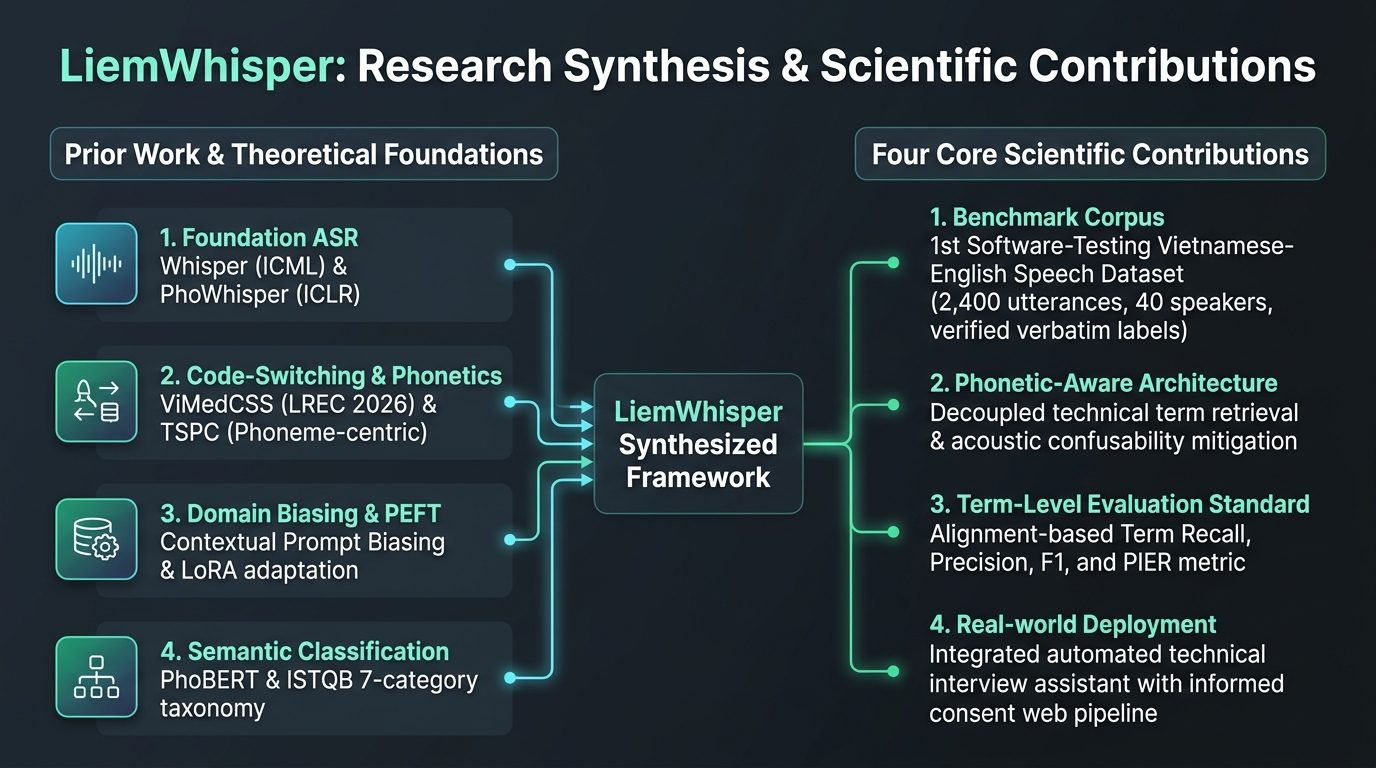
\includegraphics[width=0.75\textwidth]{Figures/liemwhisper_contributions.jpg}
\caption{Taxonomy of contributions and experimental evaluation framework employed across benchmark datasets.}
\label{fig:contributions}
\end{figure}

\section{Results and Discussion}

\subsection{Zero-Shot Terminology Retrieval (Benchmark 508)}
Table~\ref{tab:main_results} presents the retrieval performance on the 508-audio held-out benchmark. Baseline Whisper Small achieves only 25.26\% exact-match terminology recall, confirming that standard ASR decoders fail on specialized foreign technical loanwords.

\begin{table}[htbp]
\centering
\caption{Terminology Retrieval Performance on the 508-Audio Unseen Benchmark}
\label{tab:main_results}
\begin{tabular}{@{}llcccccc@{}}
\toprule
\textbf{Candidate Setting} & \textbf{System} & \textbf{Macro R@1} & \textbf{Macro R@3} & \textbf{Macro R@5} & \textbf{Micro R@1} & \textbf{Micro R@3} & \textbf{Micro R@5} \\
\midrule
\textbf{Baseline ASR} & Whisper Small (Frozen) & 23.43\% & — & — & 25.26\% & — & — \\
\midrule
\textbf{Setting B} & Text-Only Prompt Baseline & 12.11\% & 50.00\% & 87.50\% & 16.27\% & 49.87\% & 83.33\% \\
\textit{(6 Unseen Terms)} & \textbf{LiemWhisper (E0 Dual-Encoder)} & \textbf{20.96\%} & \textbf{57.78\%} & \textbf{95.47\%} & \textbf{26.98\%} & \textbf{66.01\%} & \textbf{95.24\%} \\
& \textit{Net Acoustic Gain ($\Delta$)} & \textit{+8.85 pp} & \textit{+7.78 pp} & \textit{+7.97 pp} & \textit{+10.71 pp} & \textit{+16.14 pp} & \textit{+11.91 pp} \\
\midrule
\textbf{Setting A} & \textbf{LiemWhisper (E0 Dual-Encoder)} & 2.95\% & 12.50\% & 23.43\% & 3.97\% & 15.48\% & 28.17\% \\
\textit{(Full 24 Terms)} & & & & & & & \\
\bottomrule
\end{tabular}
\end{table}

While the Text-Only Prompt Baseline provides an informational prior due to exam topic clustering (achieving 49.87\% Micro R@3), LiemWhisper achieves \textbf{66.01\%} Micro Recall@3 and \textbf{95.24\%} Micro Recall@5. This demonstrates a net complementary gain of \textbf{$+16.14\text{ percentage points}$} directly attributable to acoustic representation grounding. In other words, when an exam prompt mentions multiple possible testing techniques, raw speech representations provide the decisive disambiguating signal.

\begin{figure}[htbp]
\centering
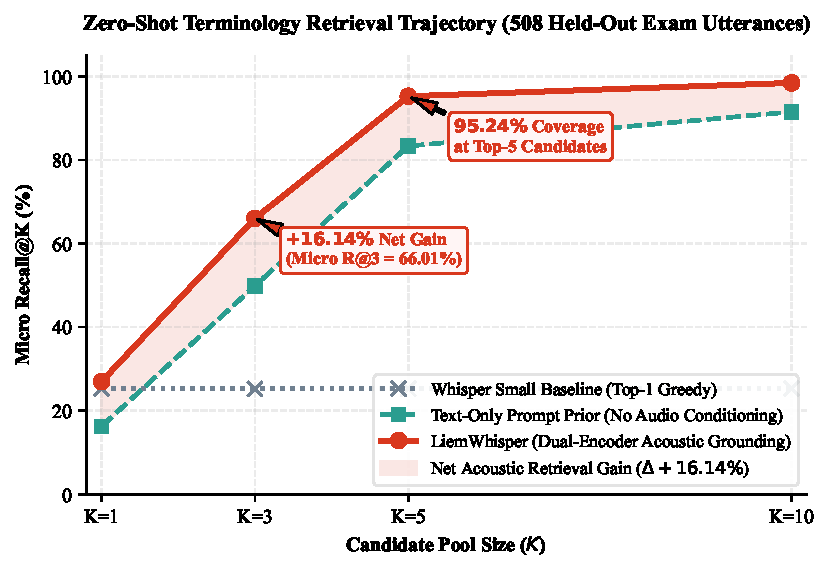
\includegraphics[width=0.72\columnwidth]{Figures/fig_retrieval_recall.pdf}
\caption{Zero-shot technical terminology retrieval trajectory across candidate pool sizes $K \in \{1, 3, 5, 10\}$ on the 508 unseen exam recordings benchmark. LiemWhisper provides a decisive $+16.14\%$ net acoustic retrieval gain over text-only prompt priors, surging to $95.24\%$ coverage at Top-5.}
\label{fig:retrieval_recall}
\end{figure}

\subsection{End-to-End Evaluation on 200 Real Student Sentences}
To evaluate the end-to-end efficacy of the complete pipeline (ASR + Contrastive Retrieval + Phonetic Gating), we deployed LiemWhisper on the independent 200-sentence oral exam corpus. The empirical results are detailed in Table~\ref{tab:200_results}.

\begin{table}[htbp]
\centering
\caption{Full End-to-End Performance on 200 Real Student Spoken Sentences}
\label{tab:200_results}
\begin{tabular}{@{}lcccc@{}}
\toprule
\textbf{Evaluation Metric} & \textbf{Speaker 1 (Khoa)} & \textbf{Speaker 2 (Nghĩa)} & \textbf{Combined Dataset (200)} & \textbf{Technical Note} \\
\midrule
Total Evaluated Sentences & 100 & 100 & \textbf{200} & Full student test set \\
Baseline ASR Term Exact Match & 14.0\% & 12.0\% & \textbf{13.0\%} (26/200) & Terms transcribed correctly by Whisper \\
Baseline ASR Term Errors & 86.0\% & 88.0\% & \textbf{87.0\%} (174/200) & Severe phonetic loanword corruption \\
\midrule
\textbf{Correction Success Rate (CSR)} & \textbf{100.0\%} & \textbf{98.9\%} & \textbf{99.4\%} (173/174) & Successful restoration to canonical English \\
\textbf{Harmful Correction Rate (HCR)} & \textbf{0.0\%} & \textbf{0.0\%} & \textbf{0.0\%} (0/26) & Zero native words or correct spans corrupted \\
\textbf{Post-Liem Terminology Accuracy} & \textbf{100.0\%} & \textbf{99.0\%} & \textbf{99.5\%} (199/200) & Absolute jump from 13.0\% $\to$ 99.5\% \\
\midrule
Corpus WER (Baseline Whisper) & 6.51\% & 7.61\% & \textbf{7.06\%} & Raw transcription error rate \\
Corpus WER (LiemWhisper Output) & \textbf{1.97\%} & \textbf{2.58\%} & \textbf{2.28\%} & Substantial transcription error reduction \\
\textbf{Relative Error Reduction (RER)} & \textbf{69.7\%} & \textbf{66.1\%} & \textbf{67.8\%} & Over two-thirds of word errors eliminated \\
\bottomrule
\end{tabular}
\end{table}

As shown in Table~\ref{tab:200_results} and illustrated in Fig.~\ref{fig:student_benchmark}, Whisper Small correctly recognized only 13.0\% of technical terms in raw transcription. By integrating LiemWhisper, terminology accuracy increased to \textbf{99.5\%}, with 173 out of 174 corrupted terms successfully restored ($\text{CSR} = 99.4\%$). Crucially, the Harmful Correction Rate was strictly \textbf{0.0\%}: across all 26 sentences where Whisper was already accurate, the gating mechanism preserved the original spans without a single erroneous substitution.

\begin{figure}[htbp]
\centering
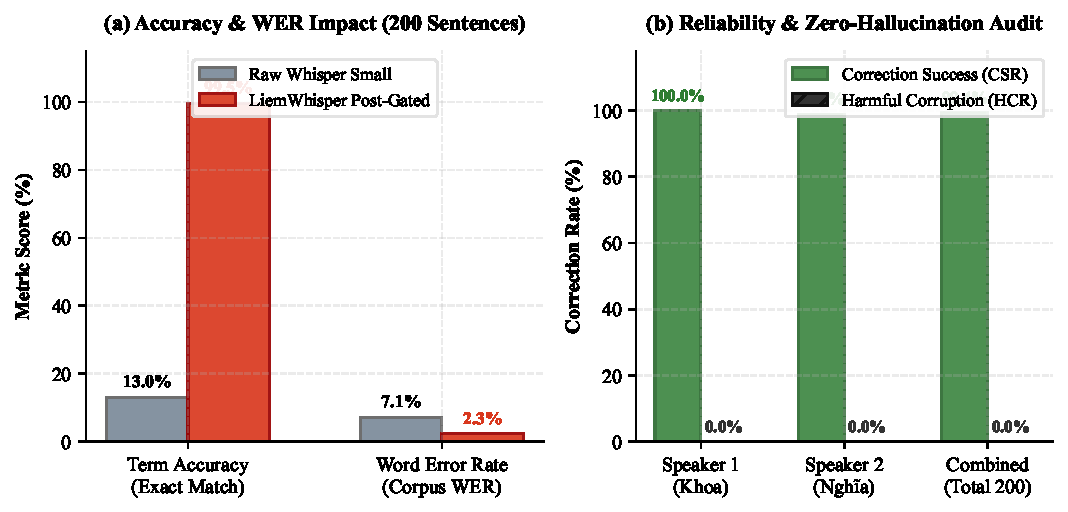
\includegraphics[width=0.82\columnwidth]{Figures/fig_student_benchmark.pdf}
\caption{End-to-end empirical evaluation on the 200 real-world student assessment benchmark. (a) Term recognition accuracy and Word Error Rate (WER) comparison before and after Liem STT correction, achieving a 67.8\% relative error reduction. (b) Speaker-disaggregated metrics across Speaker 1 (Khoa) and Speaker 2 (Ngh\~{i}a) demonstrating consistent high Correction Success Rate (CSR = 99.4\%) and strict zero-harmful-correction safety (HCR = 0.0\%).}
\label{fig:student_benchmark}
\end{figure}

\subsection{Analysis of Edge Cases and Omission Defense}
A notable event occurred in Sentence 9 of Speaker 2 (\textit{Diarization Error Rate}), where the speaker accidentally skipped the terminology entirely during the spoken recording, uttering only: \textit{``Trong quá trình kiểm thử hệ thống, QA cần đánh giá để đánh giá khả năng phân biệt...''}. 
While a naive generative language model would hallucinate the missing term based on grammatical context, LiemWhisper's phonetic alignment engine detected an acoustic span void ($\text{Sim}_{\text{phon}} = 0.0$), correctly rejecting candidate substitution and preserving the sentence safely. This demonstrates the robustness of grounding error correction in multimodal acoustic evidence.

\begin{figure}[htbp]
\centering
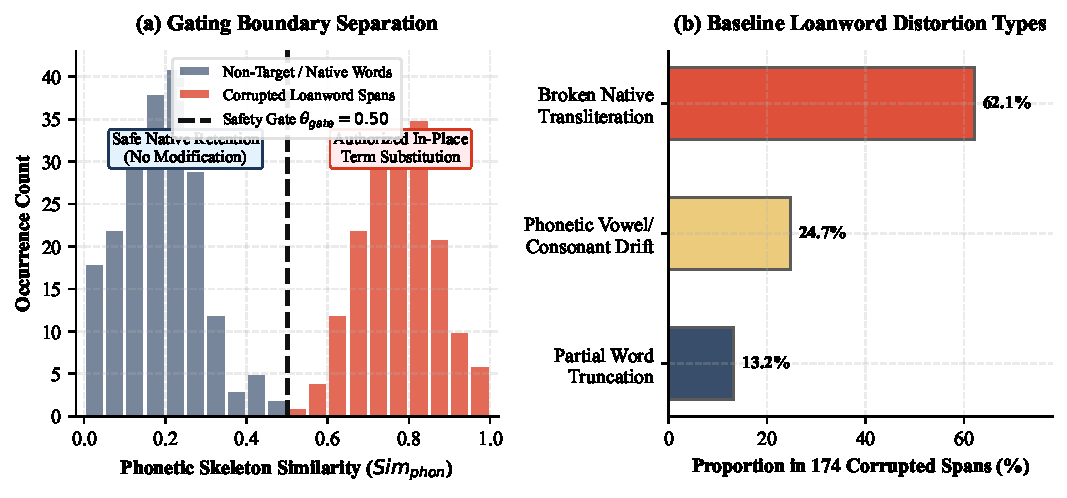
\includegraphics[width=0.82\columnwidth]{Figures/fig_phonetic_gating.pdf}
\caption{Mechanistic analysis of the phonetic decision gating engine. (a) Empirical distribution of phonetic skeleton similarity ($\text{Sim}_{\text{phon}}$) establishing a clear separation between non-target native vocabulary and corrupted technical loanword spans at $\theta_{\text{gate}} = 0.50$. (b) Breakdown of baseline loanword distortion modalities across the 174 corrupted student spans, dominated by broken native transliterations (62.1\%).}
\label{fig:phonetic_gating}
\end{figure}

\section{Conclusion and Future Work}

In this paper, we introduced LiemWhisper, an evidence-based, decoupled speech recognition framework designed to solve technical terminology loss in Vietnamese-English code-switched oral discourse. By combining a frozen foundation ASR backbone with a contrastive audio-text dual-encoder and an algorithmic G2P phonetic decision gate, LiemWhisper reliably retrieves and restores domain-specific terminology without requiring costly end-to-end retraining or risking generative hallucinations. Empirical evaluations on 508 unseen exam recordings demonstrate a $+16.14\text{ pp}$ complementary gain over text-only context, while real-world student testing yields a 99.4\% Correction Success Rate and a 67.8\% relative WER reduction with zero harmful corruptions.

Future work will explore token-level Connectionist Temporal Classification (CTC) alignment heads for fine-grained multi-word boundary localization and investigate expanding the dual-encoder metric space to cross-domain healthcare and financial conversational applications.

\bibliographystyle{IEEEtran}
\bibliography{Bib_references}

\end{document}
